%----------------------------------------------------------
\documentclass[a4paper, english, 12pt, twoside, titlepage]{article} %two-sided
\usepackage{babel, fancyhdr, amsmath, amsfonts, amssymb, graphicx, float, enumerate, hyperref}
\usepackage[utf8]{inputenc}
\usepackage[portrait,pdftex]{geometry}
%Theorem and definitions formatting
\usepackage{amsthm}

%prettier references
\usepackage{natbib}

\usepackage[autostyle]{csquotes}

% To use appendix envoronment
\usepackage[title,titletoc]{appendix}
%nomenclature
\usepackage{nomencl}
\makenomenclature
\renewcommand{\nomname}{List of abbreviations and definitions}

%used to get  figure, table and equation-numbers show the section they belong to, like ``Figure 2.1``
\numberwithin{figure}{section}
\numberwithin{table}{section}
\numberwithin{equation}{section}

%nicer captionsv
\usepackage[font=small,format=plain,labelfont=bf,up,textfont=it,up]{caption}
\usepackage{fancyhdr}
\setlength{\headheight}{15pt}

% Regluar style, with top and bottom rulers, section name at top
% and title and page number at bottom, set up for two-sided printing
\fancypagestyle{mystyle}{
	\fancyhf{} % remove everything
	\fancyhead[RO,LE]{\nouppercase\leftmark} %section name in lowercase
	\fancyfoot[LO]{\mytitle} %Title of paper
	\fancyfoot[RE]{Stud.techn. \myauthorA, Stud.techn. \myauthorB} % Name of author
	\fancyfoot[LE,RO]{\thepage} % Print page number
	\renewcommand{\headrulewidth}{0.5pt} % Ruler at top
	\renewcommand{\footrulewidth}{0.5pt}% Ruler at boottom
	\addtolength{\headheight}{15pt} % make space for the rule
}

% Plain style, just page number, set up for two-sided printing
\fancypagestyle{plain}{ %
	\fancyhead{} % get rid of headers on plain pages
	\renewcommand{\headrulewidth}{0pt} % and the line
	\fancyfoot{} % get rid of footers on plain pages
	\renewcommand{\footrulewidth}{0pt} % and the line
	\fancyfoot[LE,RO]{\thepage} % Print page number
}

% this package adds clickable links to http addresses and footnotes
\usepackage{hyperref}

%set links to be painted in black
\hypersetup{colorlinks,
linkcolor=black,
filecolor=black,
urlcolor=black,
citecolor=black}

% this package makes url's breakable with hyperref (but loses the cyan boxes)
\usepackage{breakurl}
\usepackage{multirow}
\usepackage{subfigure}

% Change margins for two-sided
\oddsidemargin 1.0cm
\evensidemargin 0.0cm

% Define aothor and title
\newcommand{\myauthorA}{Teodor Ande Elstad}
\newcommand{\myauthorB}{Simen Haugerud Granlund}
\newcommand{\mytitle}{Utilizing general-purpose computing on graphic processing units (gpgpu) for engineering algorithm speed up}

%Style to definition and RQ's
\newtheoremstyle{def}% name
  {.5\baselineskip\@plus.2\baselineskip\@minus.2\baselineskip}% Space above
  {.5\baselineskip\@plus.2\baselineskip\@minus.2\baselineskip}% Space below
  {\slshape}% Body font
  {\parindent}%Indent amount (empty = no indent, \parindent = para indent)
  {\bfseries}%  Thm head font
  {.}%       Punctuation after thm head
  { }%      Space after thm head: " " = normal interword space;
        %       \newline = linebreak
  {}%       Thm head spec


\theoremstyle{def}
% Define definition label
\newtheorem{mydef}{Definition}

% Define reserch question label
\newtheorem{myrq}{RQ}
\usepackage[parfill]{parskip}

%to include pdf
\usepackage{pdfpages}

%To inclode source code filed
\usepackage{listings}
\newcommand\pythonexternal[1]{{
\pythonstyle
\lstinputlisting{#1}}}

% Python environment
\lstnewenvironment{python}[1][]
{
\pythonstyle
\lstset{#1}
}
{}

% Python environment
\lstnewenvironment{bash}[1][]
{
\pythonstyle
\lstset{#1, language=bash}
}
{}

% Clisp environment
\lstnewenvironment{clisp}[1][]
{
\lstset{#1,language=Lisp}
}
{}

% josn environment
\lstnewenvironment{json}[1][]
{
\lstset{#1,language=json}
}
{}

% Default fixed font does not support bold face
\DeclareFixedFont{\ttb}{T1}{txtt}{bx}{n}{12} % for bold
\DeclareFixedFont{\ttm}{T1}{txtt}{m}{n}{12}  % for normal

% Custom colors
\usepackage{color}
\definecolor{deepblue}{rgb}{0,0,0.5}
\definecolor{deepred}{rgb}{0.6,0,0}
\definecolor{deepgreen}{rgb}{0,0.5,0}

% Python style for highlighting
\newcommand\pythonstyle{\lstset{
language=Python,
basicstyle=\ttm,
breaklines=true,
otherkeywords={self},             % Add keywords here
keywordstyle=\ttb\color{deepblue},
emph={MyClass,__init__},          % Custom highlighting
emphstyle=\ttb\color{deepred},    % Custom highlighting style
stringstyle=\color{deepgreen},
showstringspaces=false            %
}}
%Json Syntax
\lstdefinelanguage{json}{
    basicstyle=\normalfont\ttfamily,
    numberstyle=\scriptsize,
    stepnumber=1,
    numbersep=8pt,
    showstringspaces=false,
    breaklines=true,
}
%---------------------------------------------------------
\begin{document}

\pagestyle{empty}
%!TEX root = ../main.tex
\begin{titlepage}

\newcommand{\HRule}{\rule{\linewidth}{0.3mm}} % Defines a new command for the horizontal lines, change thickness here

%----------------------------------------------------------------------------------------
% HEADING SECTIONS
%----------------------------------------------------------------------------------------
\textsc{\large Norwegian University of Technology and Science}\\[0.2cm] % Name of your university/college
\slshape{\normalsize Faculty of Engineering Science and Technology}\\[0.1cm] % Major heading such as course name
\slshape{\normalsize Department of Engineering Design and Materials}\\[0.1cm] % Minor heading such as course title

%----------------------------------------------------------------------------------------
%	TITLE SECTION
%----------------------------------------------------------------------------------------

\HRule[0.4cm]
{ \LARGE \bfseries \textup{\mytitle}}\\[0.4cm] % Title of your document
\HRule[1.5cm]

%----------------------------------------------------------------------------------------
%	AUTHOR SECTION
%----------------------------------------------------------------------------------------

\begin{minipage}{0.4\textwidth}
\begin{flushleft} \small
\emph{Author:}\\
{\myauthorA} \\
{\myauthorB} \\
\phantom{A}
\end{flushleft}
\end{minipage}

\begin{minipage}{0.4\textwidth}
\begin{flushright} \small
\emph{Supervisors:} \\
Ole Ivar Sivertsen, NTNU \\% Supervisor's Name
Alok Mathur, Technosoft Inc \\
Bjørn Haugen, NTNU \\
Adel Chemaly, Technosoft Inc \\
\end{flushright}
\end{minipage}\\[7cm]

%----------------------------------------------------------------------------------------
%	DATE SECTION
%----------------------------------------------------------------------------------------

{\large \today}\\[3cm] % Date, change the \today to a set date if you want to be precise

%----------------------------------------------------------------------------------------
%	LOGO SECTION
%----------------------------------------------------------------------------------------

% 
\includegraphics[scale=0.5]{./gfx/ntnu_logo.eps}\\[1cm] % Include a department/university logo - this will require the graphicx package

%----------------------------------------------------------------------------------------

\vfill % Fill the rest of the page with whitespace

\end{titlepage}

\newpage

% A blank page to let the paper start on an odd-numbered page
\mbox{}
\newpage

% Roman numerals (I,II,II..) for the first pages
\pagenumbering{roman}
% Plain Style (only print page number)
\pagestyle{plain}

%

\includepdf[fitpaper=true, pages={1,2}]{assignment.pdf}
\newpage
% %!TEX root = ./main.tex


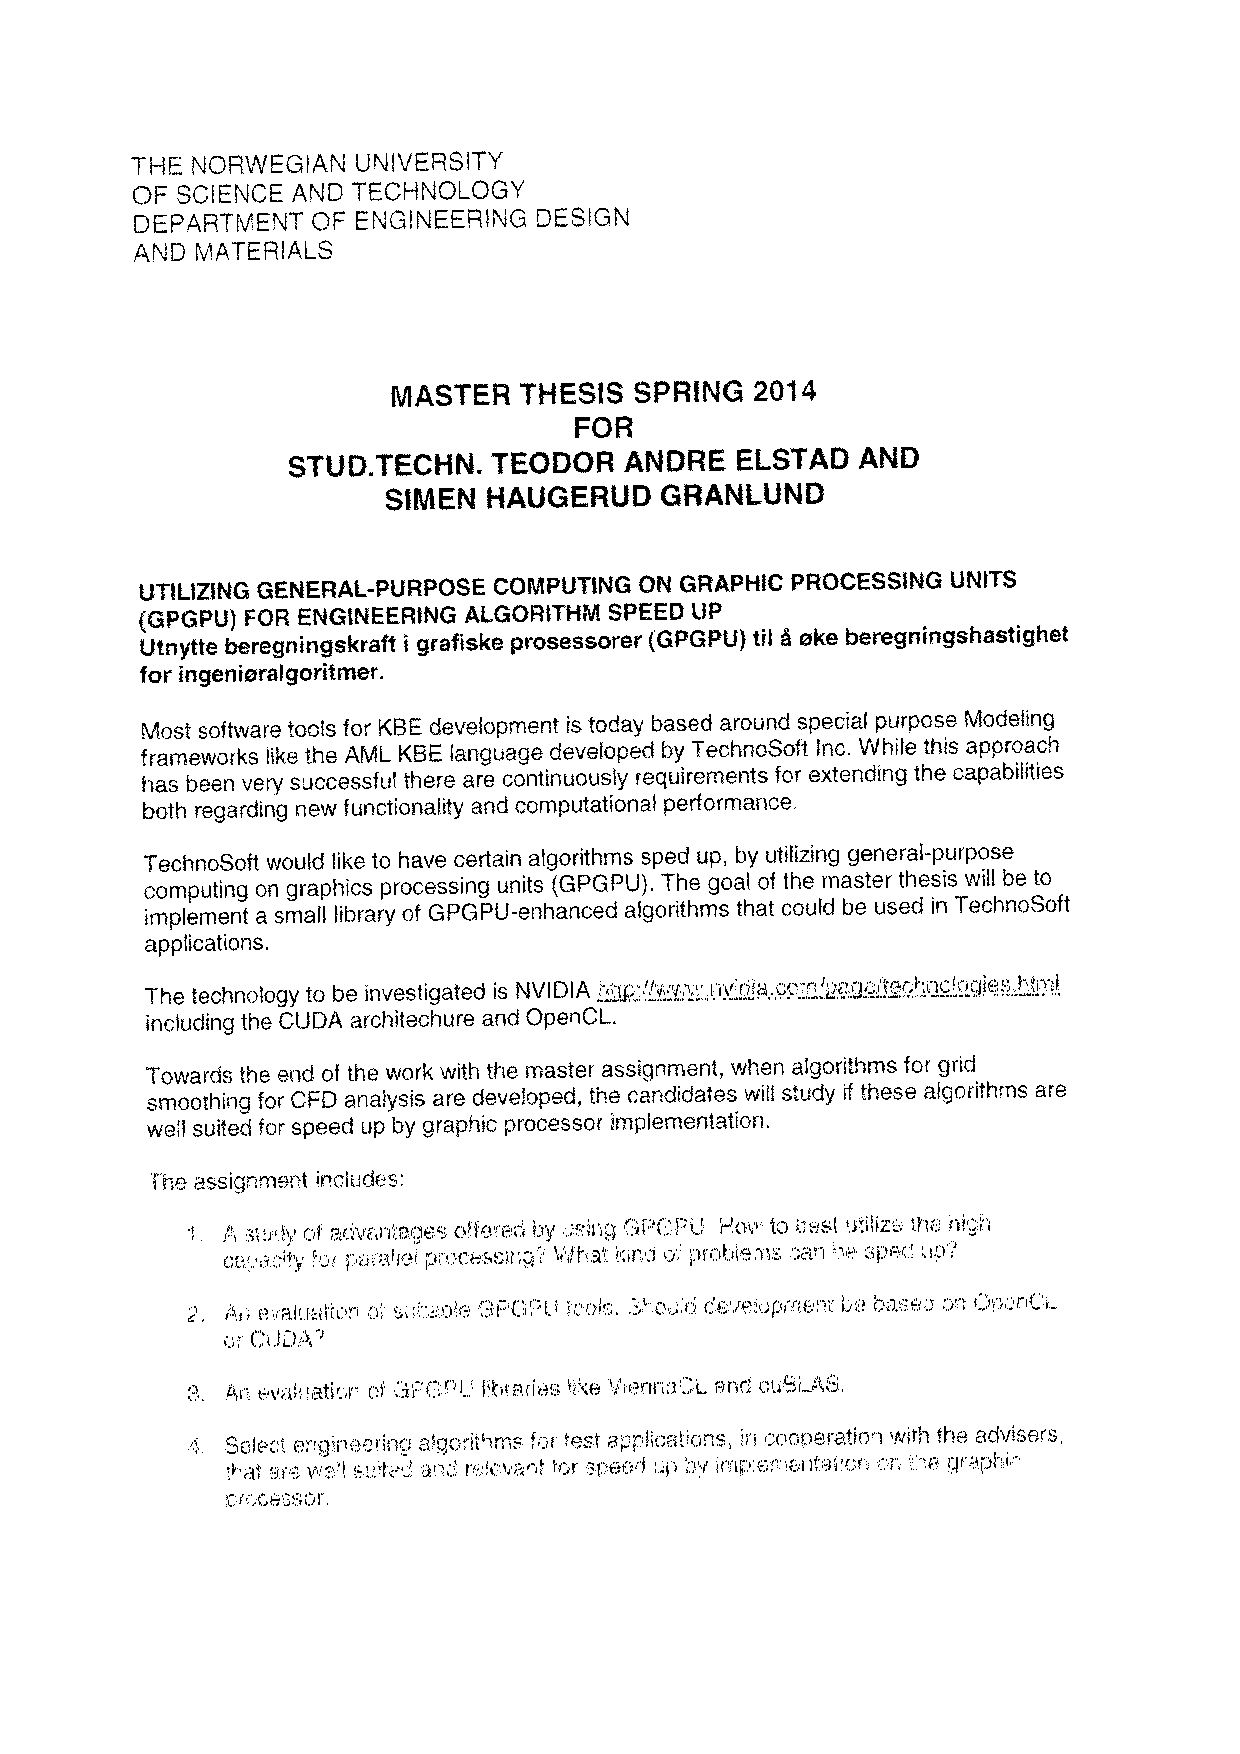
\includepdf[fitpaper=true, pages={1,2}, scale=1, noautoscale]{../gfx/assignment.pdf}
\newpage

% \section*{Assignment}

% \paragraph{} % (fold)
% Most software tools for KBE development is today based around special purpose Modeling frameworks like the AML KBE language developed by TechnoSoft Inc. While this approach has been very successful there are continuously requirements for extending the capabilities both regarding new functionality and computational performance. TechnoSoft would like to have certain algorithms sped up, by utilizing general-purpose computing on graphics processing units (GPGPU). The goal of the master thesis will be to implement a small library of GPGPU-enhanced algorithms that could be used in TechnoSoft applications. The technology to be investigated is NVIDIA http://www.nvidia.com/page/technologies.html including the CUDA architechure and OpenCL. Towards the end of the work with the master assignment, when algorithms for grid smoothing for CFD analysis are developed, the candidates will study if these algorithms are well suited for speed up by graphic processor implementation.
% % paragraph (end)

% \paragraph{The assignment includes:} % (fold)
% \label{par:the_assignment_includes_}

% % paragraph the_assignment_includes_ (end)
% \begin{itemize}
% \item A study of advantages offered by using GPGPU. How to best utilize the high capacity for parallel processing? What kind of problems can be sped up?
% \item An evaluation of suitable GPGPU tools. Should development be based on OpenCL or CUDA?
% \item An evaluation of GPGPU libraries like ViennaCL and cuBLAS.
% \item Select engineering algorithms for test applications, in cooperation with the advisers, that are well suited and relevant for speed up by implementation on the graphic processor.
% \item Extensive performance testing of different implementations on different problem sizes and hardware. Are we getting good speed up on real life problems and hardware, or is the overhead associated with parallel computing hampering performance?
% \end{itemize}

% \newpage

% The abstract page (included)
%!TEX root = ../main.tex
\begin{center}
{\Large\bfseries \mytitle}
\end{center}

\begin{center}
{\bfseries\slshape Project assignment TDT4560}
%\end{center}
\\[1.0cm]
{\bfseries\slshape
Stud.techn. \myauthorA, Stud.techn. \myauthorB \\}
Department of Engineering Design and Materials \\
Faculty of Engineering Science and Technology\\
Norwegian University of Science and Technology
\end{center}
\section*{Abstract}

The goal of this report, is to investigate the possible benefits of using general purpose software tools as a part of KBE development.

The report focuses mainly on two cases. The first case, is the possibility of extending the AML modeling framework, by interfacing with another general purpose language. By finding strategies for doing this, we are able to build a working prototype integration of the AML framework into the Sublime Text 2 editor.

The second part, explores general software tools more freely, as the possibility of building KBE models from the general purpose programming language Python is explored. This strategy gives easy integration with general software tools, and we are able to explore their benefits without the need to integrate the tool into an existing KBE development system.

Finally, the authors conclude that extending a KBE systems with modules form general software tools is beneficial, but enabling the KBE developer to extend the AML modeling framework, would be more efficient if some changes where made to AML.

\newpage


% The preface page (included)
%!TEX root = ./main.tex
\section*{\Huge Preface}
\addcontentsline{toc}{chapter}{Preface}
$\\[0.5cm]$

\noindent This thesis is based on work conducted by Stud.techn. \myauthorA and \myauthorB in the spring of 2014, as a part of a collaboration between the department of Engineering Design and Materials, Norwegian University of Science and Technology, and TechnoSoft Inc.

\noindent The authors would like to thank Professor Ole Ivar Sivertsen and Alok Mathur at Technosoft Inc. for help, guidance, feedback and inspiration throughout the project, as well as Associate Professor Bjørn Haugen and Adel Chemaly at Technosoft Inc. for their support.


\vspace*{\stretch{1}}

Trondheim, \today

\vspace*{\stretch{1}}

\rule{10cm}{0.5pt}\\
\indent \myauthorA, \myauthorB \\

\cleardoublepage

\newpage

% Prints nomenclature, to change the title of this edit
% the \renewcommand{\nomname}{List of abbreviations and definitions} in the preamble
\printnomenclature
\newpage

% Table of contents, includes only section and subsection
\setcounter{tocdepth}{2}
\tableofcontents

% List figures and tables
\newpage
\listoffigures
\listoftables

% Assure that the main content starts on an odd-numbered page
\cleardoublepage

% Use arabic (1,2,3) page numbering
\pagenumbering{arabic}

% Custom style, print name, title, section name and page number
\pagestyle{mystyle}

% include chapters
%!TEX root = ./main.tex
\section{Background}

\subsection{Introduction to the real world problem} % (fold)
\label{sub:introduction_to_the_real_world_problem}


\subsection{A short introduction to the kNN algorithm} % (fold)
\label{a_short_introduction_to_the_kNN_algorithm}

\cite{Garcia2010} In this paper a good introduction to kNN, and some relevant citations are made.

Include a transition into the TSI usecase. Fixed 3D points, large volume of repeated queries on large point cloud.

% subsection a_short_introduction_to_the_kNN_algorithm (end)


\subsection{A short introduction to relevant parallel programming principles} % (fold)
\label{sub:a_short_introduction_to_relevant_parallel_programming_principles}

% subsection a_short_introduction_to_relevant_parallel_programming_principles (end)

\subsection{A short introduction to GPU programming and CUDA} % (fold)
\label{sub:a_short_introduction_to_gpu_programming_and_cuda}

Moore's law has been a gift to all programmers the past 50 years. The law predicts that performance of integrated circlets would double every two years.Resulting in automatically faster algorithms without any work. However, since the so called Power Wall in 2002, the world has been changing. The performance boost  in processors, and verification of Moore's law, is no longer limited to a single processor core, but to multiple cores. As a result, all programs and algorithms has to be rewritten to follow the multi-core evolution.



Since the Power Wall a lot of work have been done regarding parallel programming tools, like OpenMP, CUDA, MPI and OpenCl. These tool have a varied types of supported architectures. OpenMP supports a shared memory architecture, where all cores have access to the same memory. It is an implementation of multi threading whereby a master thread divide the workload to different forked slave threads. MPI (Message Passing Interface) is a library specification for message passing, and is proposed as a standard by a broadly based committee of vendors, implementors and users. It is mostly used for communication between processors running in a distributed memory system, as most supercomputer clusters are designed today. MPI is therefore the most used parallel computer method used on supercomputer clusters today.
% An application build on both OpenMp and MPI are called a hybrid. They are used on systems that use distributed memory across different nodes, where each node uses a shared memory architecture.  These applications use MPI to send data to each node and OpenMP on individually nodes.


Although supercomputers are fast and can have thousands of cores, they are highly expensive and are not accessible for a normal consumers. Out of the current consumer level products, GPU's represent the most extreme in parallelized hardware. NVIDIA GeForce GTX, for example, can execute 23,040 threads in parallel, and in practice requires at least 15,000 threads to reach full performance \citep{karras2012}. The reason GPU's have such a massive amount of parallelized threads if that each thread is very lightweight. The benefit is that together they can achieve extremely high instruction throughput. This makes the GPU perfect for high performance computing.


\subsubsection{General-purpose computing on graphics processing units} % (fold)
\label{ssub:general_purpose_computing_on_graphics_processing_units}


The GPU's extreme properties and the highly increasing interest in multi core systems have also made the General-purpose computing on graphics processing units (GPGPU) programming landscape rapidly evolve. GPGPU is the utilization of GPU in applications, to perform heavy computation, that is normally handled by the CPU. Several new programming approaches have appeared and a convergence to a standardized model has began. Two widely used approaches are Compute Unified Device Architecture (CUDA) and The Open Compute Language (OpenCL).


OpenCl is a low-level framework for heterogeneous computing on for example CPU and GPU's. It includes a programming language, based on C99, for writing kernels. Kernels are methods that executes on the GPU. It also includes an API that are used to define and control the platform.

In contrast to the open OpenCL, the dominant proprietary framework is CUDA. It is, as OpenCL, based on a programming language and a programming interface. Science CUDA is created by the vendor, it is developed in close proximity with the hardware.

% subsubsection general_purpose_computing_on_graphics_processing_units (end)

\subsubsection{NVIDIA GPU architecture} % (fold)
\label{ssub:nvidia_gpu_architecture}


The biggest difference between a GPU and a CPU is there primal objective. The CPU is optimized for low latency, while the GPU is optimized for high throughput. For a chip to achieve low latency it needs to have ha huge amount of cache available, which makes it harder to fit a lot of cores. To get high throughout a lot of cores or ALUs are needed. The GPU has therefore a small control unit and cache, but is packed with cores. Basically we can say that the difference is how the transistors are used. The GPU has more transistors dedicated to computation, then the CPU.

At the hardware level, a NVIDIA GPU is build around a scalable array of multithreaded Streaming Multiprocessors (SMs). A multiprocessor are designed to execute hundreds of threads concurrently. It is organized according to an architecture called SIMT (Single-Instruction, Multiple-Thread), where each SMs creates, manages, schedules and executes parallel threads in groups of 32. This is called a warp. Threads composing in a warp starts at the same program address, but they have their own register state and instruction address, and is therefore free to branch and execute independently \citep{cuda_programming_guide}.

An other impotent part of the GPU architecture is the memory hierarchy. Global memory is bottom-most part of this hierarchy and is analogous to RAM on the CPU. The global memory can be used to transfer memory to and from the host CPU. Each SM contains a fast shared memory, which is shared across each thread in the SM. The threads also have their own 32-bit registers. There also exists other types of memory, called constant memory and texture memory. Compared to the CPU, the peak floating-point capability and memory bandwidth of the GPU, is an order of magnitude higher \citep{LiangcuKnn}.


% subsubsection nvidia_gpu_architecture (end)

\subsubsection{CUDA programming model} % (fold)
\label{ssub:cuda_programming_model}

The CUDA programming model is designed to make the heterogeneous GPU+CPU programming easier. The GPU works as a computation accelerator for the CPU, and the programming model should therefore be an easy bridge between the two. CUDA have created this bridge based on a runtime library, compiler and C language extensions. The C language extensions enables the programmer to create and launch methods on the GPU, through the runtime library. These methods are called kernels.

A CUDA program is is based on a data-parallel behavior, where threads is running in parallel. The execution of a kernel is organized as a grid of blocks consisting of threads. When a kernel grid is launched, on the host CPU, blocks of the grid is enumerated and distributed among the SMs. The blocks then executes concurrently on individual SMs. As blocks terminates, new blocks are added. Only threads in a block can communicate with each other, by creating synchronization walls. They can also communicate through the fast shared memory, that is located on each individual SM. Each block and thread have their own id, which often is used to determines what portion of data to be processed by each thread.

% subsubsection cuda_programming_model (end)

%!TEX root = ../main.tex
\section{Evaluation of generic software development tools} % (fold)
\label{sec:evaluation_of_generic_software_development_tools}
In this chapter, we will look at some of the different tools used for GSD, and specify a set of tools we will focus our following investigation on.

\subsection{Currently used GSD tools} % (fold)
\label{sub:currently_used_gsd_tools}
In this section we will try to list some of the tools, currently used for GSD. Due to the large amount of different tools available, we do not aim to make an exhaustive list. Instead we will focus our list of tools associated with the popular Agile method for development , as well as a section of well used traditional tools, used for software development.

There is two reasons for focusing on Agile development tools. The first is the popularity of using this method has in GSD. The second is that using agile principles with KBE, is a practice currently being developed and utilized buy AkerSolutions KbeDesign. The benefits of such tools have already been studied by both AkerSolutions and Lars Barlindhaug in his thesis \citep{aunit}, and the fact that tools for agile development is currently being in development, makes interesting to study the possibility of integrating ready-made solutions from the world of GSD.

Agile development has introduced a lot of new development tools. Tools like unit test frameworks, which enables the developer to run the same tests over and over again. Mock frameworks, which simplifies and standardizes the test writing. Test runners, which allows tests to be automated \citep{agile_samurai} \citep{Martin:2008:CCH:1388398}. Alongside tools for testing, agile projects often utilize tools for continuous integration (CI). CI is the process of automating the building and testing process in software development, and in this thesis Lars Barlinghaug showed the feasibility and relevance of such practices in an KBE environment \citep{aunit}.

Although Agile development is currently receiving a lot of attention in the GSD community, the use of support tools in GSD is not limited to the tools associated with agile development. One of the most overlooked tool is the editor or IDE the developer uses to write the code. The general practice in GSD is that several editor options exist for every programming language, all though some might be better suited than others.

Debugging tools, which allow the developer to step through the execution of the program and inspect variable instantiation, is a common support tool. The value of being able to perform such inspections on a KBE model

The use of previously written modules and libraries, is also a practice, widely used in GSD. Using previously written code, makes development faster and less error prone. This is not a new concept for KBE development, indeed AML facilitates the creation of reusable modules and libraries to a great extent. Would it be possible to also use modules and libraries from the larger GSD community? This could hypothetically extend the choices of the KBE developer, something that makes this an interesting case to study.

IDE or editor used to write the code is an essential tool. This is an interesting case to study, since XEmacs currently is the only editor currently supported by the popular AML modeling framework. Could other editors of IDEs bring new features to AML?

An often overlooked tool, that all software developers use at some point, it the tools available for learning a particular software system. This is especially relevant for a KBE system, Rocca states that: the role of KBE developer should be easily undertaken by engineers and not restricted to ‘‘natural born hackers’’ \cite{rocca}. Good learning tools is a part of making this possible. This is of particular interest to the writers, as we will have to undergo training in AML as a part of the project.
% subsection currently_used_gsd_tools (end)

\subsection{Tools studied in this project} % (fold)
\label{sub:tools_studied_in_this_project}
Due to time constraints, we will not be able to study all the possible GSD tools relevant for KBE development. In this section we will give a brief argument for why we have chosen to study certain tools.

The tools for Agile development, is of particular interest, due to the investigation made by AkerSolution and Lars Barlindhaug, and we will focus on integration of previously written tools for testing.

Using modules and libraries from a GSD language is also something that we'll study. KBE development is a relatively smaller field than GSD, and as a result there is fewer ready-made components to choose from. Enabling the KBE developer to access a much larger amount of previously written components. This will require us to study the possibilities for integrating with AML from other programming languages.

Integrating AML with another editor is also something that we'll study. The lack of several supported code editing tools for AML is puzzling, as a large amount of code editing options are available for GSD. Integrating AML with another code editing tool, will also serve as a test of the strength of our findings in how to interface with AML.

Finally we'll look at the possibility of using a debugger in KBE development. A debugger is a feature which is lacking from AML, but is widely used in most of GSD.
% subsection tools_studied_in_this_project (end)
% section evaluation_of_generic_software_development_tools (end)

%!TEX root = ../main.tex

\section{Extending AML} % (fold)
\label{sec:extending_aml}

\subsection{Interfacing with the AML modeling framework} % (fold)
\label{sub:interfacing_with_the_aml_modeling_framework}
In order to be able to extend the AML modeling framework, without writing every extension from the ground up, we need to understand how we can interact with AML from other applications. In this section we will look at how to control AML from other applications. We will first discuss control through the console, and then through the use of sub-processes in Python.

\subsubsection{Interfacing with AML from the console} % (fold)
\label{ssub:interfacing_with_aml_from_the_console}
Using the console is a simple but powerful way to control a computer. Not only can the user give complex instructions in a short and concise manner, these instructions can be automated through batch-scripting, the resulting batch-files can be executed from other programs. Commands and results can even be streamed from one program to another. Although not the norm for consumer applications, a solid command line interface is the standard for GSD tools.

In this section we will compare the AML command line interface with the command line interface of comparable general purpose programming languages. We will identify similarities and features suitable for improving the AML command line experience.

We started our investigation by searching for documentation on using AML as a command line tool. This topic is not covered in the AML basic training \citep{aml_ref} and we where unable to get hold of such documentation from Technosoft. This was unfortunate, as we had to base our investigation on previous work done by Olivier \citep{olivier}, reverse engineering of the existing start-up batch-files supplied with AML, as well as a good bit of experimentation.

To investigate AML as a command line tool, we choose two simple tasks, launching and interacting with the interpreter from the command line, as well as running a previously written program, and displaying the results in the command line. This would be compared with the procedures for accomplishing the same tasks with Common Lisp (in the form of the CLISP implementation) and Python.

Common Lisp and Python are good languages to compare AML against, as both features an interpreter, and relies heavily in this feature for development. Common Lisp is also interesting, because it shares the same syntax as AML. Python does not share the syntax, but is also implemented by using the C programming language. Let's start out by looking at how the two tasks are preformed by the CLISP and Python interpreter.

Depending on the installation and underlying operating system, you start the interpreters in any directory by simply typing \texttt{clisp} or \texttt{python} into the command line. On Windows systems, you sometimes have to to specify the path to the interpreter executable file in the environment variables to make the executable reachable from any directory. This is dependent on the installer, as some might set this variable as a part of the installation process.

Interacting with the interpreter is then as simple as writing commands in the command line, and executing them with return. Examples of launch and use of Python and CLISP is shown in Listing~\ref{lst:multiLinePython} and Listing~\ref{lst:multiLineClisp}.

\begin{python}[caption={Use of the Python interpreter},label={lst:multiLinePython}]
teodoran@HAL:~$ python
Python 2.7.4 (default, Sep 26 2013, 03:20:26)
[GCC 4.7.3] on linux2
Type "help", "copyright", "credits" or "license" for more information.
>>> def greetProfessor(name):
...     print("Good day professor " + name)
...
>>> greetProfessor("Ole-Ivar")
Good day professor Ole-Ivar
\end{python}

\begin{clisp}[caption={Use of the  the Clisp interpreter},label={lst:multiLineClisp}]
teodoran@HAL:~$ clisp

Welcome to GNU CLISP 2.49 (2010-07-07) <http://clisp.cons.org/>

(Copyright statements omitted)

Type :h and hit Enter for context help.

[1]> (defun greet-teacher-assistant (name)
(format t ``I promise I'll deliver the assignment soon ~s!'' name))
GREET-TEACHER-ASSISTANT
[2]> (greet-teacher-assistant ``Jens'')
I promise I'll deliver the assignment soon ``Jens''!
NIL
\end{clisp}

In the case of a malformed statement, both interpreters return the error message and stack trace directly into the command line. CLISP even supports injection of new code, instead of the erroneous code, through the use of restarts.

To start AML in the console, a minimal environment has to be set up. This is sometimes performed by a included batch script. A version of this script, describing the required setup, is shown in Listing~\ref{lst:amlStartup}

\begin{bash}[caption={AML5-startup-win32.bat},label={lst:amlStartup}]
ECHO OFF

SETLOCAL

set "AML_TRAINING_ROOT=%CD%\"
set "AML_STARTUP_DIR=%AML_TRAINING_ROOT%AML-Startups\AML-Startup-Win32\"
set "AML_DIR=%AML_TRAINING_ROOT%AML\AML5_Win32\"

cd %AML_STARTUP_DIR%
"%AML_DIR%AML.exe" "%AML_DIR%aml.img"

ENDLOCAL
\end{bash}

The startup script initiates a few variables needed by the AML process. Then it launches AML.exe with the AML.img file.

This gives us an running AML interpreter, that functions much in the same way as the CLISP and Python interpreter. Errors also gives rise to a pop-up dialog, where the user can choose to debug or abort. Choosing the debug option, prints the stack trace to the console.

Using a pop-up dialog to display debug information might have its benefits in a GUI setting, but as a part of a command line interface, it can cause some troubles. If the user where to use the program remotely with a networking interface without graphical forwarding, like ssh without X11 forwarding, the open dialog would cause the AML interpreter to hang indefinitely.

Using a interpreter in this fashion is a quite common occurrence in the general software world. You might have a centralized testing or deployment server set up, where accessing and running code remotely would be beneficial. It also makes batch-scripting with AML more prone to fatal errors, as the script has no way to know if something went wrong with the AML process.

Over to the task of running previously written programs. With CLISP or Python, this is performed by executing the program with the program piped through standard in. This code can be piped directly from a source file, or from the output of another program. Listing~\ref{lst:executingPython} and Listing~\ref{lst:executingClisp} shows how this is done for Python and CLISP respectively.

\begin{bash}[caption={Executing Python},label={lst:executingPython}]
teodoran@HAL:~$ python print-ta.py
Teacher assistant
\end{bash}

\begin{bash}[caption={Executing Clisp},label={lst:executingClisp}]
teodoran@HAL:~$ clisp print-professor.lisp
"Professor"
\end{bash}

Running previously written AML-programs is a bit more laborious. You can load and compile systems on startup by editing the logical.pth file or you can load or compile you system with commands directly in the AML interpreter.

The problem with the available options for running previously written programs with AML, is that it makes it harder to automate tasks with batch scripts, since the batch-process cannot interact with the interpreter after it is launched. This makes executing AML programs seemingly unnecessary hard, and during our experimentations, we have not been able to perform this task.
% subsubsection interfacing_with_aml_from_the_console (end)

\subsubsection{Running AML from another application} % (fold)
\label{ssub:running_aml_from_another_application}
One way of handling programming language interoperability, is to let one language execute code in the other, by using subprocesses. A classic example is an application interfacing with a relational database, through execution of SQL-statements. This is by no means the only way to handle programming language interoperability. Another way is using languages that can be compiled into the same executable code, .Net being the famous example of this approach, and it is an approach that makes one language interface with a very different one. In this sections we will investigate the possibilities for controlling the AML framework through subprocesses in another language.


The case used for this investigation will be a REPL application (Read Eval Print Loop), written in Python, that implements the full functionality of the AML interpreter. The user should be able to launch the Python application, and use it as he or she would use the AML interpreter.

This is conceptually a simple problem. You query the user for input, evaluate the input through the AML-subprocess, and then print the result to the command line, before looping the sequence all over again. Pseudo-code for such an application is shown in Listing~\ref{lst:replPseudoCode}.

\begin{python}[caption={Pseudo-code for a AML REPL application},label={lst:replPseudoCode}]
while true:
    print(evalWithAMLSubProcess(readLine()))
\end{python}

Naive translation of Listing~\ref{lst:replPseudoCode} into Python code, using the Popen class to handle the subprocess, did not work, and displayed an interesting bug. The program prints out the loading statements, but hangs indefinitely when the user should be prompted for the first input. Why was this happening?

Although we cannot be absolutely certain of what has gone wrong in the previous example, since we do not have access to the AML source code, the problem shows symptoms of a known problem relating unbuffered, line buffered and fully-buffered output. In the draft for the ISO C standard N1124, we can read the following:

\begin{quote}
When a stream is unbuffered, characters are intended to appear from the source or at the destination as soon as possible. Otherwise characters may be accumulated and transmitted to or from the host environment as a block. When a stream is fully buffered, characters are intended to be transmitted to or from the host environment as a block when a buffer is filled. When a stream is line buffered, characters are intended to be transmitted to or from the host environment as a block when a new-line character is encountered. \cite{N1124}
\end{quote}

At program startup, three text streams are predefined and need not be opened explicitly: standard input (for reading conventional input), standard output (for writing conventional output), and standard error (for writing diagnostic output). As initially opened, the standard error stream is not fully buffered; the standard input and standard output streams are fully buffered if and only if the stream can be determined not to refer to an interactive device.

This applies to our problem. It is known that AML is implemented in C, and it is fair to assume that it uses the C standard IO library (stdio) to preform IO operations. This would not be a problem if the standard out stream was unbuffered or line buffered, since the results would have been sent for every character or line. The main problem is that the stdio library only sees that it is connected to a pipe in our program, and will therefore conclude that it is not connected to a interactive device, therefor going into a fully buffered mode. The result is that our Python program waits indefinitely for the result from the AML process.

To test this theory we ran the same example, using Python with an option to force line-buffered IO. This worked as intended.

One way to try to circumvent this problem, is by reading and writing to the AML process in two threads. Listing~\ref{lst:replThreadedPopen} shows one way op accomplishing this.

\begin{python}[caption={Python AML REPL with two threads},label={lst:replThreadedPopen}]
import subprocess
import sys
from threading import Thread

process = subprocess.Popen(['AML5-startup-Win32.bat'], shell=False, stdin=subprocess.PIPE, stdout=subprocess.PIPE)

def print_stdout():
        while process.poll() is None:
                output = process.stdout.readline()
                sys.stdout.write(output)

t = Thread(target=print_stdout, args=())
t.start()

while True:
        input = sys.stdin.readline()
        process.stdin.write(input)
        process.stdin.flush()
\end{python}

This will accomplish our task, but has the unfortunate side effect of having us manage the communication between two different threads.

Another way of accomplishing the task, is to use a pseudo-TTY. This is a program that emulates the command line environment, making the stdio library believe it is communicating with an interactive device. Developing an application that uses a pseudo-TTY requires a lot of development, or the use of a framework for pseudo-TTY work, as this is a quite complex task. Due to the difficulties in finding a suitable pseudo-TTY library for the Windows 8 operating system, the test was performed on Ubuntu 13.04, with CLISP emulating AML, by running in block-buffered mode. This test was successful.

\pythonstyle
\begin{lstlisting}[caption={Python CLISP REPL with pseudo-TTY},label={lst:replPseudoTty}]

import pexpect

c = pexpect.spawn('clisp')
c.expect('\[\d+]>')
print c.before.strip()

def evalArg(arg):
    c.sendline(arg)
    c.expect('\[\d+]>')
    return c.before.replace(arg, '', 1).strip().replace('\n', '', 1)

done = False
while not done:
    expression = raw_input('> ')

    if expression == 'exit':
        done = True
        c.sendline('(exit)')
        c.expect(pexpect.EOF)
        print c.before.replace('(exit)', '', 1)
    else:
        print evalArg(expression)
\end{lstlisting}

The benefit of this approach is the possibility of getting real interaction between the AML process and our own program, but this interaction comes with an sizable overhead and increase of complexity.
% subsubsection running_aml_from_another_application (end)
% subsection interfacing_with_the_aml_modeling_framework (end)


\subsection{Extending the development environment} % (fold)
\label{sub:extending_the_development_environment}

\subsubsection{The importance of development environment choice} % (fold)
\label{ssub:the_importance_of_development_enviroment_choice}
When developing applications in the world of general software development, you have the choice of selecting from a wide array of tools. You'll more often than not start out by determining what kind of programming language, development framework, development methodology, project organization tools, testing framework, continuous integration tool, and so forth, is most suited for the task at hand, and maybe more important, compatible with the knowledge in your team.

An important point to consider for the programmer, is the choice of development environment. Development environment is a term with different definitions, but we will define it as the software-tools used by the programmer to develop the new application, which is not part of the code-base.

\begin{mydef}
Development environment: The software-tools used by the programmer to develop the new application, which is not part of the code-base.

Software frameworks is omitted from this definition. Although software frameworks can be considered a tool for the software engineer, it becomes a part of the developed application.
\end{mydef}

The development environment forms the tools used by the software engineer to perform his or her craft. Important parts of this environment is the code editor, source control tools, project planning tools, and so on. You could even argue that the chosen operating system is a part of the development environment.

An woodworking analogy would be the tool chest. The nail and wood is not part of the development environment, as it is destined to become a part of the final product. The hammer used for hammering the nails, and the saw used for cutting the wood is a part of the development environment, and can differ from tool chest to tool chest.

A motivation for making this division, is that the choice of development environment is often partially determined by the individual programmer, and can often differ within the same development project. These choices is also a factor that'll remain constant for a programmer between projects. An simple example: a programmer can use Emacs to work on both a web-development project in Python and a email-client in C++.

One of the most important tools of the development environment is the code editor. This is the tool that enables the software engineer to write code, and although we can find no statistical study, it is safe to assume that a large amount of the software engineers workday is spent using the code editor to write code. Therefore have we chosen to focus our work on the code-editor part of the AML development environment.

Almost no other tool is at such a whim of the taste of the programmer as the code editing tool. The therm “Editor war” is well known, and so is Richard Stallman humorous “Church of Emacs” \citep{stallman}. Although there has been made endless non-constructive arguments over which editor or IDE reign supreme, we will not be discussing this. Instead we will put forth some arguments for why editor diversity is beneficial for development in AML.

\begin{itemize}
  \item Editor choice gives new KBE developers the option of choosing the editor that most closely resembles a editor they are familiar with, in effect reducing the training time.

  \item A choice of editor, makes AML less dependent on one editor technology. If the dominant editor style where to change in the future, AML would be more ready to support such a change. This is indeed a case of today, where programmers is moving from simple text-editors to integrated development frameworks (IDE's).

  \item Exposing AML to different development environments gives the AML-developer access to the different features of the different development environments associated with each editor.

  \item Choice is freedom for the developer. A trait that is usually cherished by today's software developers.
\end{itemize}

There is an argument to be made against supporting multiple editors for AML, in that it it steals valuable development resource from the core functions of AML. This is a big concern, because a KBE-vendor should be able to focus on delivering the best tools for KBE-development, not code-editing. But is it possible to have the best of both worlds? Can the relationship between the AML-development environment and the code editor be structured in such a way that it is easy to maintain for the vendor, yet enables the developer to use his favorite editor of choice? This is indeed the case with general software development today, where most programming systems can be used with any number of development environments. Our hypothesis will therefore be that this is possible for AML development as well.

\begin{myrq}
\label{rq:structure_aml}
    It is possible to structure the relationship between the AML-development system and the code editing tool, in such a way, that it is possible to use other editors than XEmacs, with a minimum of development and maintenance.
\end{myrq}

We will also investigate the new features integrating another code editor gives to the AML development environment.

\begin{myrq}
\label{rq:another_editor}
    Can another editor, give access to other development environment features, not readily available in XEmacs.
\end{myrq}

We will investigate these questions by trying to integrate the AML development framework with the Sublime Text 2 editor, and we will briefly review the work made by Oluf Tonning \cite{oluf} on integrating AML with Eclipse and Olivier Doucet \cite{olivier} on integrating AML into the .Net framework.
% subsubsection the_importance_of_development_enviroment_choice (end)

\subsubsection{Features of an AML editor} % (fold)
\label{ssub:features_of_an_aml_editor}
Let's start our investigation by looking at the most important features of the current XEmacs integration, and try to organize the features by importance to the programmer. We will then try to divide our findings into features that should be part of the AML integration and features that are related to the editor choice.



\begin{description}
    \item[AML console:] At the center of the XEmacs is the AML console. The console allows the developer to interact with the running AML process through a REPL interface in one of the emacs buffers. The developer is, amongst other, able to compile and run code, interact with the compiled models and send commands to the AML system.

    \item[Launch of AML GUI:] This can be performed directly in the AML console by using the \texttt{(aml)} command, but GUI elements for performing this is also present.

    \item[AML Documentation:] GUI elements give direct access to the AML manual by opening the manual in the default web browser.

    \item[AML syntax highlighting:] The XEmacs integration features Lisp-style syntax highlighting, as well as highlighting of some AML-specific expressions.

    \item[AML code completion:] Code completion can be performed through XEmacs extensive macro system, but no default completions are included. Dynamic abbreviation, completion of words previously written in any open buffer, is supported and can be accessed by pressing {M - /}.

    \item[AML code navigation:] The XEmacs integration features ILISP-like code navigation (a well known emacs major mode for editing Lisp, \cite{cliki}, superseded by SLIME, the Superior Lisp Interaction Mode for Emacs). Most notable is the possibility to search for definitions of functions from anywhere in the project.

    \item[AML code formatting:] Auto-formatting of sections of code in standard Lisp style is supported, although on a side note, lines with lone right parentheses is encouraged in the AML documentation. This is in direct conflict with general Lisp style guides, as documented by both the GNU Emacs Lisp coding conventions, \cite{gnu} and the Google style guide for Common Lisp, \cite{google}.
\end{description}

We can categorize these features into two groups. The first group is the features strictly unique to the AML development framework. The second is features that is more general in nature, and could be implemented by using existing editor functionality or plug-ins from the general software development community.

The AML console, launch of the AML GUI and the AML documentation is features which are unique to AML, but the syntax highlighting, code completion, navigation and formatting are features that closely resembles general editor features for Lisp-like languages. We note that launch of the AML GUI is a sub function of the AML console. If the AML console is implemented, will launch of the AML GUI be possible.

Access to the AML documentation is of also of a lower importance. Opening a local web page is something a developer would be able to do, even if there was no explicit GUI functionality for doing so in the editor. Geir Iversen \cite{geir} could also inform us that this is the preferred way to use the AML manual at Aker Solutions KBeDesign.

This implies that a basic integration of AML into any editor consists of two parts:

\begin{enumerate}
    \item Integrating the AML console into the chosen editor.
    \item Configure relevant existing Lisp-editing tools and plug-ins to work with AML.
\end{enumerate}

This strategy already has its merits. Oluf Tonning \cite{oluf} used this strategy to successfully integrate the AML development framework into the Eclipse IDE. Although this integration never gained major use, due to the quality of the Lisp support in Eclipse \cite{geir}, it remains an important proof of concept.

Based on the previous discussion, we can evaluate existing code-editing tools for AML integration suitability. We will include categories for console support, Lisp support, as well as general configurability, since this will be important in configuring the editor for a new language. We will also consider user-friendliness for beginner programmers, since \enquote{KBE development should not only be for natural born hackers} \cite{rocca}. The results of this evaluation can be found in Table \ref{tab:editorEval}.

\begin{table}
    \begin{center}
        \begin{tabular}{| l | l | l | l | l |}
            \hline
            Editor/IDE & Console support & Lisp support & Configurability & Beginner friendly \\ \hline
            Visual Studio & Yes & Low & Medium & Medium \\ \hline
            Eclipse & Yes & Medium & Medium & Medium \\ \hline
            Emacs & Yes & High & High & Low \\ \hline
            Vim & Yes & High & High & Low \\ \hline
            Sublime Text & Yes & High & High & High \\ \hline
        \end{tabular}
    \end{center}
    \caption{Editor/IDE evaluation}
    \label{tab:editorEval}
\end{table}

Based on the evaluation and our familiarity with the editor, we chose to base further work on Sublime Text 2 (Sublime Text version 2).
% subsubsection features_of_an_aml_editor (end)

\subsubsection{Configuration of existing Lisp tools in Sublime} % (fold)
\label{ssub:configuration_of_existing_lisp_tools_in_sublime}
The first step was to configure existing Lisp support tools for use with AML. This is done through the existing package support in Sublime. A new folder was made for AML, and the existing configuration for Common Lisp was included. In addition code completion snippets for AML KBE classes was made. This gave the editor satisfactory syntax highlighting and, combined with the default dynamic abbreviation in Sublime, code completion features.

The default editor provided good code navigation by default, except for the possibility of searching for function definitions. Some auto formatting features was also included by default, but these features was found to be insufficient.

Sublime features an extensive library of open source, third party plug-ins. Installation and maintenance of these features is most easily organized through Sublime Package Control \citep{bond}.

To enhance auto-formatting, the package Sublime Lispindent \citep{Friberg}, was installed. Testing revealed this plug-in to give good results by re-using the default configuration for Common Lisp as shown in Listing~\ref{lst:lispindentConfig}.

%TODO fjerne syntax on the word self.
\begin{lstlisting}[language=json, caption={Lispindent config},label={lst:lispindentConfig}]
"aml": {
    "detect": ".*\\.(aml)$",
    "default_indent": "function",
    "regex":        ["(catch|defvar|defclass|
        defconstant|defcustom|defparameter|
        defconst|define-condition|define-modify-macro|",
        "defsetf|defun|defgeneric|define-setf-method|
        define-self-expander|defmacro|defsubst|deftype|
        defmethod|",
        "defpackage|defstruct|dolist|dotimes|lambda|
        let|let\\*|prog1|prog2|unless|when)$"]
}
\end{lstlisting}

The indentation behavior of Lispindent can also be modified through regex parameter in the config file, although this was never desired in our tests.

In order to enable search for function definitions, the package Find Function Definition \citep{Douglas}, was added. This enables the developer to highlight a function name, and search for the corresponding definition in the current project by pressing F8. The plug-in will display a list of files to open if multiple instances of possible definitions is found.

This plug-in also required a minimal setup to work with AML, and the setup can be extended to include other syntactic elements, like classes.

\begin{lstlisting}[language=json,caption={Find Function Definition Config},label={lst:findFuctionDefinitionConfig}]

{
    "definitions": /* where $NAME$ is the name of the function */
    [
        "function $NAME$",
        "$NAME$: function",
        "$NAME$:function",
        "$NAME$ = function",
        "$NAME$= function",
        "$NAME$=function",
        "def $NAME$(",
        "(defun $NAMES$"
    ]
}
\end{lstlisting}
% subsubsection configuration_of_existing_lisp_tools_in_sublime (end)


\subsubsection{Integration of the AML console} % (fold)
\label{ssub:integration_of_the_aml_console}
Based on the discussion under Section~\ref{ssub:running_aml_from_another_application}, we choose to base our console integration on the multi-threaded approach. The code for this integration is found in Appendix~\ref{sec:amlrepl}. A pseudo-TTY approach would be better, but the added complexity would mean that we would not be able to even remotely argue for the integration being easy to maintain and develop.

A approach based on an AML-process in unbuffered or line buffered mode would have been even better, as there exist ready made tools for integrating such interpreters into Sublime \cite{bederski}.

The problems with having to juggle two different threads became apparent when implementing the AMLRepl. In order for the main thread to be able to access the write out from STDOUT, the reading thread had to write the lines into a global variable. The main thread would the try to check at regular interval for new out-print in this global variable, and clearing it after writing the content to the text buffer.

This is not the most elegant solution, and regularly requires the user to force an out-print of the global variable with the command Ctrl + Alt + w.

Sending code to the AML interpreter was, on the other hand, an easy job. The open API of Sublime made it an breeze to get the wanted code from the text buffers.

Some design choices where made in regards to the functionality of the REPL. One was to try to maintain as much of the default editing capabilities of the text-buffer containing AMLRepl. This meant that we would keep the default behavior of the return key. Instead we ended up using \texttt{Ctrl + Return} as our default evaluate expression key.

Since the Lisp syntax is so easy to parse, we made the default evaluate expression function to look for the last complete Lisp expression in the current file. This behavior can be overridden, by first marking the desired statements to evaluate. Entire files can also be evaluated by pressing Ctrl + Alt + e.
% subsubsection integration_of_the_aml_console_ (end)

\subsubsection{Additional Configuration} % (fold)
\label{ssub:additional_configuration}
A couple of additional features was added, once the basic editing and REPL functionality was in place. The first one to be added was functions for launching the AML GUI. This was simply done by using the existing functions to make a function that always would send (AML) to the interpreter.

Using the same approach launch of AUnit, the AML unit test framework, was integrated into Sublime. This required a bit more setup, since the logical.pth file has to include the AUnit paths, as shown in Listing~\ref{lst:aunitLogicalPth}.

\begin{lstlisting}[caption={Aunit logical path},label={lst:aunitLogicalPth}]
:aunit                "<full-path-to-sublime-text-folder> ...
                    ... \Data\Packages\AMLRepl\AUnit\src\"
:aunit-main-system    :aunit main\
:aunit-core-system    :aunit core\
:aunit-print-system   :aunit print\
:aunit-gui-system     :aunit gui\
\end{lstlisting}

%TODO: edit (anuint) and(comple-system)
The AUnit system can then be compiled and launched using the (compile-system ...) and (aunit) functions.

We hoped to be able to display test results from AUnit directly in another text-buffer, as this would have given a more seamless integration. The developer would then have been able to edit, execute and test the AML code, using only the Sublime interface, and the AML GUI where graphical inspection was needed. This should have been possible, due to AUnit being developed with a command line mode \cite{aunit}. Unfortunately our version of AUnit had a bug in the command line functionality, and coupled with project time constraints, this was never realized.

Finally the different functions of the integrations was made available through menu entries and the command palette, as well as being available directly from shortcuts.

User configurable parameters was bundled together into suitable JSON configuration files, accessible from the settings menu. Readme-files, describing basic use and installation was also added.
% subsubsection additional_configuration (end)

\subsubsection{Notable differences between Sublime and XEmacs} % (fold)
\label{ssub:notable_differences_between_sublime_and_xemacs}
As stated in the introduction, we will not argue for one editor over another, as we believe that preference of one editor over another is largely due to taste and familiarity. Although the main benefit of integrating AML into Sublime is to give the developer several options to choose from, some notable features of Sublime should be mentioned.

\begin{itemize}
    \item AML console: At the center of the XEmacs is the AML console. The console allows the developer to interact with the running AML process through a REPL interface in one of the emacs buffers. The developer is, amongst other, able to compile and run code, interact with the compiled models and send commands to the AML system.

    \item Sublime has a more modern GUI, with a tab system that closely matches modern tabbed applications, like web browsers. This is a interface that younger developers is more familiar with, and might make the editor learning process easier.

    \item Sublime is customized by using the widely used general programming language Python. This will make customization of the editor easier for developers familiar with Python, as they do not have to learn the lesser known Emacs Lisp language.

    \item The command palette, gives the developer access to all the options and commands available in Sublime, by utilizing fuzzy search. This makes it easy to find features and commands for the beginner, as well as lesser used features and commands for the experienced user.

    \item Sublime has a more modern default key-binding, familiar from most other applications. One example is Ctrl-c for copy and Ctrl-v for paste.

    \item Browsing and editing the project files and folders can easily be done in the left side bar of the editor.

    \item Sublime has a large and active plug-in community. This gives the developer access to , easily installed to the Sublime package manager.

    \item The minimap on the right side of the editor, gives the developer an instant overview of the open file. This is especially useful when editing large files.
\end{itemize}
% subsubsection notable_differences_between_sublime_and_xemacs (end)
% subsection extending_the_development_environment (end)

\subsection{Learning material} % (fold)
\label{sub:learning_material}
The learning material is often the first part of a programming system the developer experiences. For complex tools, like AML, it plays a large role in making the tool easy to use.

When debugging an error, you do not have a good reference to the error messages. For most general software development tools, you can simply search for the error text to get a better explanation. This is also something that could be covered in the training documents.

We have, in retrospect, evaluated our learning experience with AML. Technosoft delivers the AML Basic Training Manual \cite{aml_ref}. This manual is meant as a complete, beginners course to AML. The manual tries to cover the most important features of AML, mostly by following a case, concerning the aerodynamic surfaces of a missile. In addition, Technosoft delivers AML with a manual \cite{AML}. The manual is meant as an documentation of all the features available in AML, and although examples and explanation to the different language constructs are given, it's focus is on being a reference manual, not a training text.

Our experience with the reference manual was that it has two major strong-points. The first is it being a web-page with an exhaustive index. Chapters on different subjects can be opened in different browser tabs, and terms can be searched for by using the browser command find on the index page. The organization of the different terms also feels natural, and makes it easy to find related terms to the terms you already know. The second strong-point is the examples. As well as efficiently displaying the usage of the language term, it is a great starting point for further exploration in the AML interpreter. In our opinion even more examples would have been a useful addition to the reference manual.

The basic training manual left us with the impression that in the effort of trying to cover all aspects of AML, it does not manage to cover each section with enough depth. More intermediate and advances examples are not given not given enough space, and as a result, developing real world KBE-applications is a big step after finishing the manual. This we felt, was especially a problem when covering the topics relating to general use of a programming language with Lisp syntax.

The most dominating programming languages today, Java, C\#, C++, and so on, uses C-derived syntax, quite different from the Lisp syntax of AML. Concepts as cons cells as the underlying data structure, functions as data, immutable variables, dynamic typing and macro programming is fundamental to Lisp programming, but does not play a big part in the C-derived languages. To gain a bigger understanding of these concepts, we turned to learning material for Common Lisp.

Another factor in efficient training, is the possibility of getting several different explanations of the same topic. While you might not understand a given language concept with one explanation, several explanations from different point of view might help you to form an understanding. We used the following resources when learning to use AML.

\begin{itemize}
    \item Land on Lisp by Conrad Barski \cite{landoflisp}.

    \item Practical Common Lisp by Peter Seibel \cite{practicalcommonlisp}.

    \item On Lisp by Paul Graham \cite{Graham.1994}.

    \item Common Lisp hyperspec \cite{www.lispworks.com}.
\end{itemize}

Our experience was that the lessons learned form working with Common Lisp, translated well into working with AML. The basic syntax was very similar, and most basic examples could be compiled as AML. Although small syntactic differences was still an annoyance when they arose.

Looking at the learning material for general programming languages, we can find a lot of interactive tutorials. Some good examples are Codecademy \cite{codecademy}, Try Clojure \cite{tryclojure} and Learn Knockout.js \cite{learnknockoutjs}. Common for all the learning resources is that they bundle code editing, compilation and a step by step tutorial text into the same interface. The user is guided step by step through different tasks, first being explained the concept and then advancing when they supply the correct code to the given problem, or choose to be shown the solution.

Such an interactive learning experience might be interesting to explore with AML, and should be able to implement in both the Sublime and Emacs editor.

The most popular general software programming languages usually have active on-line communities. The communities discuss use of the language, improvements, solutions to common problems and is often a place for beginners to get answers and guidance. Some communities use on-line forums or maintain sites for questions and answers (QA sites). A very successful on-line community for programming language QA is the site Stack Overflow \cite{stackoverflow}. Technosoft curating such a forum or QA site, might be beneficial.
% subsection learning_material (end)
% section extending_aml (end)
%!TEX root = ../main.tex

\section{Turning the problem around} % (fold)
\label{sub:turn_the_problem_around}

There are several ways to integrate general software tools in KBE development. One way, is to make the KBE tools adapt to the rest of software development environment. This way, all ready-made and future-make general software tools, can be used in KBE development without major adapting work. The KBE environment will naturally follow the evolution in software development, and can easily adapt to new changes. The KBE system vendor can focus on their core operation, and not spend time trying to adapt to the rest of the software evolution.

This idea is based one one key assumption, that it is easy to integrate general software tools in a KBE-system that is based on a general programming language. We will formulate this assumption as the following research question:

\begin{myrq}
\label{rq:intgenssofttools}
Is it easy to integrate general software tools, if a KBE-system is based on a widely used programming language?
\end{myrq}

\subsection{How to test the hypothesis?} % (fold)
\label{ssub:how_to_test_our_hypothises}
In order to begin to answer this question, we have to overcome one notable obstacle. As of today, there is no KBE-system that follows the general software evolution. The major KBE-systems use proprietary languages like GDL, IDL and AML. These languages are highly adapted for KBE development, but lack the great support that widely used languages have. To investigate this question, we therefore have to make a minimal KBE-system based on a general software language. Only then we can test our hypothesis.

We will therefore make a minimal KBE-system based on Python, Open CASCADE and FreeCAD. Then we will investigate if it is easy to integrate some of the general software tools that Python supports.
% subsubsection how_to_test_our_hypothises (end)


\subsection{The minimal KBE system} % (fold)
\label{sub:the_kbe_system}
In order to make a minimal KBE-system, we must understand the core features of a KBE system, and how this can be implemented. Rocca et al. investigates this as a part of the paper: \enquote{Knowledge based engineering: Between \{AI\} and CAD. Review of a language based technology to support engineering design'} \cite{rocca}. Rocca argues that a basic KBE-system contains three essential parts, a viewer, geometry kernel and a programming interface, as shown in figure \ref{fig:3parts}.

\begin{mydef}
  A minimal KBE system is build up of a geometry kernel, graphical viewer and a programming interface.
\end{mydef}

\begin{figure}[ht!]
\centering
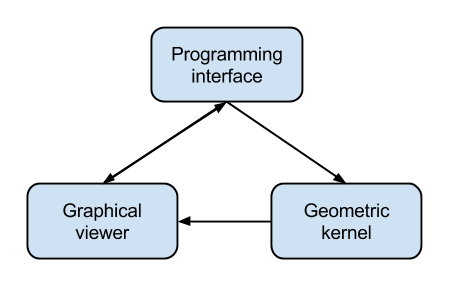
\includegraphics[width=90mm]{gfx/kbe_system_in_3_parts.png}

\caption{The tree essential parts in a KBE-system and their relation}
\label{fig:3parts}
\end{figure}

\begin{description}
  \item[The programming interface] is what makes a KBE-system special. This is where the rules governing each model is stored. It also describes the object structure needed to create the geometry. The programming interface is build up of a programming language, and must have an interface to the geometric kernel. It must also communicate with the viewer, so the viewer knows about each KBE-object, its parameters and the relation between each object.
  \item[The graphical viewer] is where the KBE-object and models can be queried and visualized. The are often tree main components.
  \begin{description}
    \item[The tree pane] shows the object hierarchy.
    \item[The inspector pane] is where the properties of a KBE-object can be viewed and manipulated.
    \item[The view-port pane] is where the KBE-model is visualized.
  \end{description}
  \item[The geometric kernel] is a 3D modeling component, which feed geometric data to the viewer, based on data received by the programming interface module.
\end{description}

The main feature of a KBE system is the programming interface. The programming interface governs the object structure, logic and control that can be implemented in the KBE model. The two other components, the graphical viewer and geometric kernel, is used in many engineering systems today and is not a unique KBE part. Many CAD systems, like NX UGS, FreeCAD and AutoCAD, use the same combination, but the KBE viewer differs in how it visualize a models meta data, and the control components. The viewer system of a KBE system and a CAD system is still comparable.
% subsection the_kbe_system (end)


\subsection{Programming interface} % (fold)
\label{sub:programming_interface}
To make a minimal KBE-system, we must first choose a suitable programming language. Today almost all KBE languages are object oriented and have some main declaration types, as shown in Table~\ref{tab:languageParts} from \cite{rocca}. Possibly the most relevant operator is the \texttt{define-class}operator, which declares a class definition. It allows defining classes, superclasses, objects and relationships of inheritance. We can organize the rest of the expressions, as ether attribute function or subclass declarations. The attributes can again be divided in default, descendant, editable or normal attributes declarations. These declarations are similar to the modern object-oriented programming paradigm, which is supported by many general purpose programming languages today. The basic concept for this paradigm, is to represent the consent of objects with attributes and methods and the relationship between these objects \citep{van_ray}s.

\begin{table}[ctb]
  \begin{center}
    \begin{tabular}{p{4cm}lp{5cm}l}
    \hline
    \textbf{GDL} & \textbf{IDL} & \textbf{Knowledge Fusion} & \textbf{AML} \\
    \hline
      define-object & defpart & defclass & Define-class \\
      input-slot & input & Any data type a followed by the behavioral flag b parameter (plus optional default value)&\\
      Input-slot:settable (or:defaulting) & Default-inputs&&\\
      computed imputs& attributes&Specification of several data types, plus an optional behavioral flag(e.g., lookup, uncached and parameter) &\\
      computed-slot:settable  &Modifiable-attributes&A data type followed by the behavioral flag modifiable&\\
      Trickle-down-slots &Descendant-attributes&All attributes descendant by default&\\
      Type &Type&Class&\\
      Objects&Parts&Child&Sub-objects\\
      Hidden-objects &Pseudo-parts& Class name starts with&\\
      Functions &Methods&Functions&\\
    \hline
    \end{tabular}
  \end{center}
  \caption{KBE language operators to define classes and objects hierarchies}
  \label{tab:languageParts}
\end{table}


\subsubsection{Essential features} % (fold)
\label{ssub:essential_features}
We see that the basic concepts of a KBE language is supported in the object-oriented paradigm \citep{rocca} with one exception. The specific attribute declaration, which describe how the attribute should be handled throughout the instantiation and inheritance procedure, is not a standard feature of most general purpose object-oriented languages. This features is handled by native declarations in most KBE languages, but this might not be a necessary feature. Controlling instantiation and inheritance procedure can be handled by creating a basic object structure. The basic object structure can then control relations like superclasses and children in the object hierarchy. It can also make the different types of attributes.

Other essential part of a KBE language, is its ability to give commands to a geometric kernel. To make this possible, an interface have to exist between the language and the geometric kernel.
% subsubsection essential_features (end)


\subsubsection{Non-essential features} % (fold)
\label{ssub:non_essential_features}
Some features make the KBE language more more flexible and controllable, but is not essential. Dynamic typing and multiple inheritance are two examples. Languages without these features are more strict, and don't support mixins, which, for example, make implementing materials and coordinate systems easier. Knowledge Fusion is one kind of KBE language that don't support these features \citep{rocca}.

Models also tend to be very large when making KBE application, which make calculation and rendering of the model time consuming. This is solved by many KBE-systems today with demand driven evaluation. Demand driven evaluation, also known as lazy evaluation, is an evaluation strategy, which delays the evaluation of an expression until its value is needed. This gives the KBE system the ability to just recalculate and render the parts needed in the model update. There are more solutions to this problem than just a native support for lazy evaluation. One solution is to implement a pattern called observable pattern. This pattern allows a one-to-one or one-to-many dependency between objects, so that when the observed object is changed in some way, all the observers can be notified \citep{rollings}.

Other notable non-essential features, are syntactic overhead and open source. Syntactic overhead is a programming languages ability to eliminate syntactic elements, unnecessary in a given problem domain. The \enquote{Hello World} example in Java exemplifies syntactic overhead. The developer has to contain the print statement in an main function and a container class, none of which serves the overarching goal of printing a string to the console. For this problem domain, printing a string to the console, Java would be considered to have high syntactic overhead. This is not always a bad feature, but using a programming languages with low syntactic overhead can mean less writing and more focus on the essential parts of the model. The benefit of open source programming languages, is that widely used open source languages often get a lot of constructive feedback from the open source community regarding bug reports and fixes, support, development of new software tools and libraries, as well as a collaborative culture. This often leads to programming languages with high quality, good documentation and a wide variety of support tools.

\begin{mydef}
  Syntactic overhead is a language ability to eliminate unnecessary syntactic elements for a given problem domain.
\end{mydef}
% subsubsection non_essential_features (end)


\subsubsection{Choosing a programming language} % (fold)
\label{ssub:choosing_a_programming_language}
We can review some key features from the discussion above, and try to evaluate what kind of programming languages that are suitable for KBE development. The result of this evaluation is shown in Table~\ref{tab:chooselanguage}. We have chosen to spit the features in essential and non-essential features. The essential features are that we regard as a \enquote{must have} feature, while non-essential features are \enquote{nice to have}. We also added one other category, which try to describe what kind of general software tools that is supported in the programming language.

\begin{table}[tb]
  \begin{center}
    \begin{tabular}{|l|c|c|c|c|c|c|}
    \hline
     \textbf{Feature}& \textbf{AML} & \textbf{Python} & \textbf{CLisp} & \textbf{C}++  & \textbf{C}\# & \textbf{Java} \\
    \hline
       \multicolumn{7}{ |l| }{\textbf{Essential features}} \\
    \hline
    Object-oriented & Yes&Yes&Yes&Yes&Yes&Yes\\
    \hline
    Interface to geometric kernel & Yes&Yes&Yes&Yes&Yes&Yes\\
    \hline
    \multicolumn{7}{ |l| }{\textbf{Non-essential features}} \\
    \hline
    Native demand driven evaluation & Yes&Yes&Yes&No&Yes&No\\
    \hline
    Dynamic typing & Yes&Yes&Yes&No&No&No\\
    \hline
    Multiple inheritance & Yes&Yes&Yes&No&No&No\\
    \hline
    Open source & N&Yes&Yes&Yes&No&Yes\\
    \hline
    Syntactic overhead & Low&Low&Low&High&Medium&Medium\\
    \hline
    \multicolumn{7}{ |l| }{\textbf{General software tools}}\\
    \hline
    Debugging tool &No&Yes&Yes&Yes&Yes&Yes\\
    \hline
    Test framework support &Low&High&Medium&High&High&High\\
    \hline
    IDE support &Low&High&Medium&High&High&High\\
    \hline
    Community &Low&High&Medium&High&High&High\\
    \hline
    \end{tabular}
  \end{center}
  \caption{A comparison table between KBE language features and some programming languages.}
  \label{tab:chooselanguage}
\end{table}

From Table~\ref{tab:chooselanguage} we can draw some conclusions. First we see that all languages is a suitable KBE language, because they all support the essential features. The specific KBE object structure and hierarchy is something that all the languages can imitate. When we look at the non-essential section, we see that some languages are more suitable than others. Common Lisp, AML and Python stand out as the three most suitable languages. They have all the features that enhance flexibility and control, like demand driven evaluation, dynamic typing and multiple inheritance. They also have a low syntactic overhead. Another ting that differentiates them is that they are open source.

Investigating the feature most relevant to our RQ~\ref{rq:intgenssofttools}, the GSD tool support, we observe that Python, C++, C\# and Java has the most support. All languages have a good and varied selection of compatible general software tools, and this makes them highly selectable for our test. The loser in this category is AML, probably due to this being a lesser used, proprietary programming language. A honorable mention is the AUnit test framework for AML, but this tool is still in development.

Based on this evaluation we choose to use Python as our base language, because it has all the features needed to become a KBE language, and has good support for general software tools, which is crucial in order to explore our research question.
% subsubsection choosing_a_programming_language (end)
% subsection programming_interface (end)


\subsection{Geometric kernel and graphical viewer} % (fold)
\label{sub:geometric_kernel_and_graphical_viewer}
A programming language alone does not make a KBE system. We still need to find a geographical viewer and a geometric kernel. Available modeling kernels compatible with Python are:

\begin{itemize}
  \item \textbf{Parasolid} by ShapeData, now owned by Siemens.

  \item \textbf{ACIS} by Spatial Corporation.

  \item \textbf{ShapeManager} by AutoDesk.

  \item \textbf{RGK} by Russian Federation's Ministry of Industry and Trade.

  \item \textbf{Open CASCADE} - by open source community.
\end{itemize}

The two most used kernels are Parasolid and ACIS, which are use by NX, AML, AutoCAD and SpaceClaim. RGK is a newly developed kernel, with a lot of positive feedback \citep{RGK}, but is still in development. The only major geometric kernel that is both proven in other applications and based on open source, is Open CASCADE and is therefore the only one economic scope of this project. It includes C++ components for 3D surface and solid modeling, visualization and data exchange.

The geometric kernel and graphical viewer has to be connected to each other and the programming language. This give some restriction in choosing the viewer component of our KBE system, since we have chosen Python as the base programming language. We are also restricted regard to development time, so a ready-make viewer and geometric kernel combination is preferable. Some open source applications satisfies our requirements:

\begin{itemize}
  \item The first option is PythonOCC \citep{OCC}. PythonOCC is an 3D CAD/CAE/PLM development framework for Python. There is no GUI component, just a Python interface to the underlying OpenCascade kernel and libraries to prototype a viewer.

  \item The second option is FreeCAD \citep{FreeCAD} and its Python objects called PytonFeatures. PythonFeatures are 100\% Python objects, and contains a visualization and geometry part. FreeCAD is a parametric 3D modeler. This makes it more similar to traditional CAD applications than PythonOCC. FreeCAD includes a built-in Python interpreter and an open API, that covers almost all features of the application. With this scripting feature, a developer is able to create an object structure, on top of the viewer and kernel, to create a KBE model.
\end{itemize}

Both these alternatives are able to give us the base of our testing platform. Both have a viewer and a geometric kernel, that is controlled by a Python API. All that is left, in order to create a KBE-model, is to create the programmable interface. Out of these two alternatives we choose FreeCAD. The main reason for this was development time, and since we only need a minimal KBE system to test our resource question (RQ~\ref{rq:intgenssofttools}), FreeCAD was the easiest application to use.
% subsection geometric_kernel_and_graphical_viewer (end)


\subsection{Creating the testing platform} % (fold)
\label{sub:the_creating_the_testing_platform}
Now we have the basic tools to create our testing platform. Before we start implementing, we need to set some restrictions on our minimal KBE system. There is no need to create a complete system to test our hypothesis, just the basic functionality.

\begin{itemize}
  \item Performance is not an issue, because we only need to make small models. Therefore we do not need to think about demand driven evaluation or other performance enhancing features.

  \item Only focus on geometry, not meshing or FEM analysis.

  \item Create a basic object structure, that support multiple inheritance and children.
\end{itemize}
% subsubsection restricting_the_test_platform (end)


\subsubsection{The object structure} % (fold)
\label{ssub:the_object_structure}
To control instantiation and relationship between each object, we have created a superclass, called KbePart (see Appendix~\ref{app:kbepart.py}). This object has to be inherited from all KBE classes. It contains a set of functions that can be used by the inherited classes, as described below.

\begin{description}
  \item[make\_properties()]  can be extended to add properties to the model.

  \item[make\_property(name, property\_type)] can be used to make a editable and descendant property. It returns a object with all editable and descendant properties.

  \item [add\_children()] is used to add and manipulate children.

  \item[make\_child()] is used to add a child.

  \item[get\_properties\_list()] return a list of all editable and descendant properties.

  \item[print\_msg()] can be used to print messages to the viewer's console pane.
\end{description}

\begin{figure}[ht!]
\centering
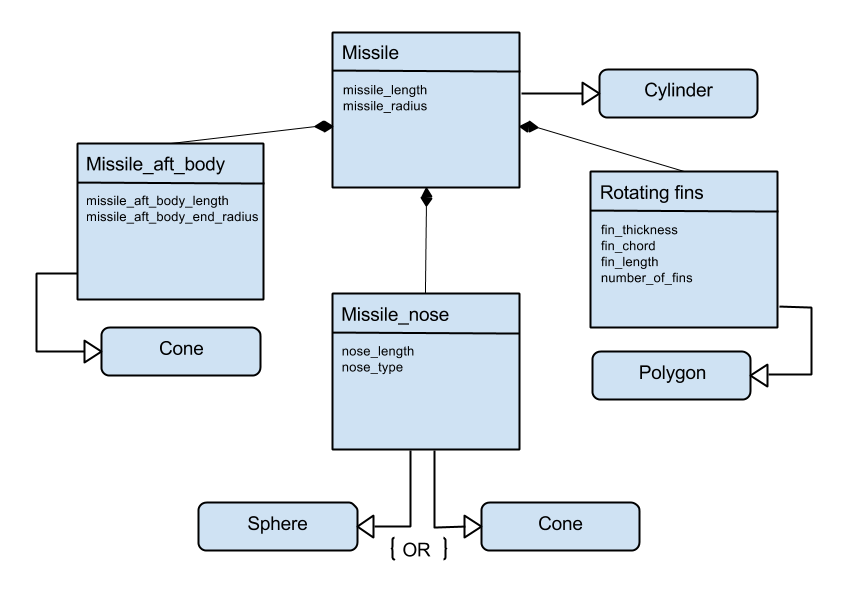
\includegraphics[width=150mm]{gfx/uml_diagram_of_missile.png}

\caption{UML Class diagram for the Missile class showing inheritance and composition links.}s
\label{fig:object_structure}
\end{figure}
% subsubsection the_object_structure (end)


\subsubsection{The test model} % (fold)
\label{ssub:the_test_model}
Based on this object structure, we have created a simple missile model (see Appendix~\ref{app:missile.py}), based on the case from the AML Basic Training Manual \cite{aml_ref}. This model is going to be used to test-environment for our hypothesis. The missile is build out of objects inherited from the KbePart. From figure~\ref{fig:object_structure}, we can see that the missile class is based on a set of other subclasses, missile\_nose, missile\_aft\_body and rotation\_fins.

From figure~\ref{fig:freecad}, we can see the graphical viewer with the three pane, editable properties pane and view-port pane. From the properties pane, we can see that all the properties have propagated from the child objects to the missile. The properties can also be edited to change the geometry of the missile.
% subsubsection the_test_model (end)
% subsection  (end)


\subsection{Integrating general software tool} % (fold)
\label{sub:integrating_general_software_tool}

Now that we have a test platform we can start integrating some general software tools. Three GSD tools, that are going to be investigated in particulare is debugging tools, tools for testing and IDE/editor support.


\subsubsection{Interfacing with FreeCAD and Open CASCADE} % (fold)
\label{ssub:Interfacing with FreeCAD}

To get Pythons general software tool to work in a FreeCAD environment, an interface need to exist between them. This interface is the Python programming language. All FreeCAD features, like modeling, meshing and simulations, are accessible thought a Python API. This makes it easy to integrate different kinds of tools. FreeCAD is imported into Python as a normal module. The process for doing this in a temporary way is shown below:

\begin{python}
import sys sys.path.append("path/to/FreeCAD/lib")
\end{python}

FreeCAD can now run inside other applications that use Python or from an external Python shell. We can also import our KbePart the same way:

\begin{python}
import KbePart
\end{python}

This makes our minimal KBE system very modular.

\begin{figure}[ht!]
\centering
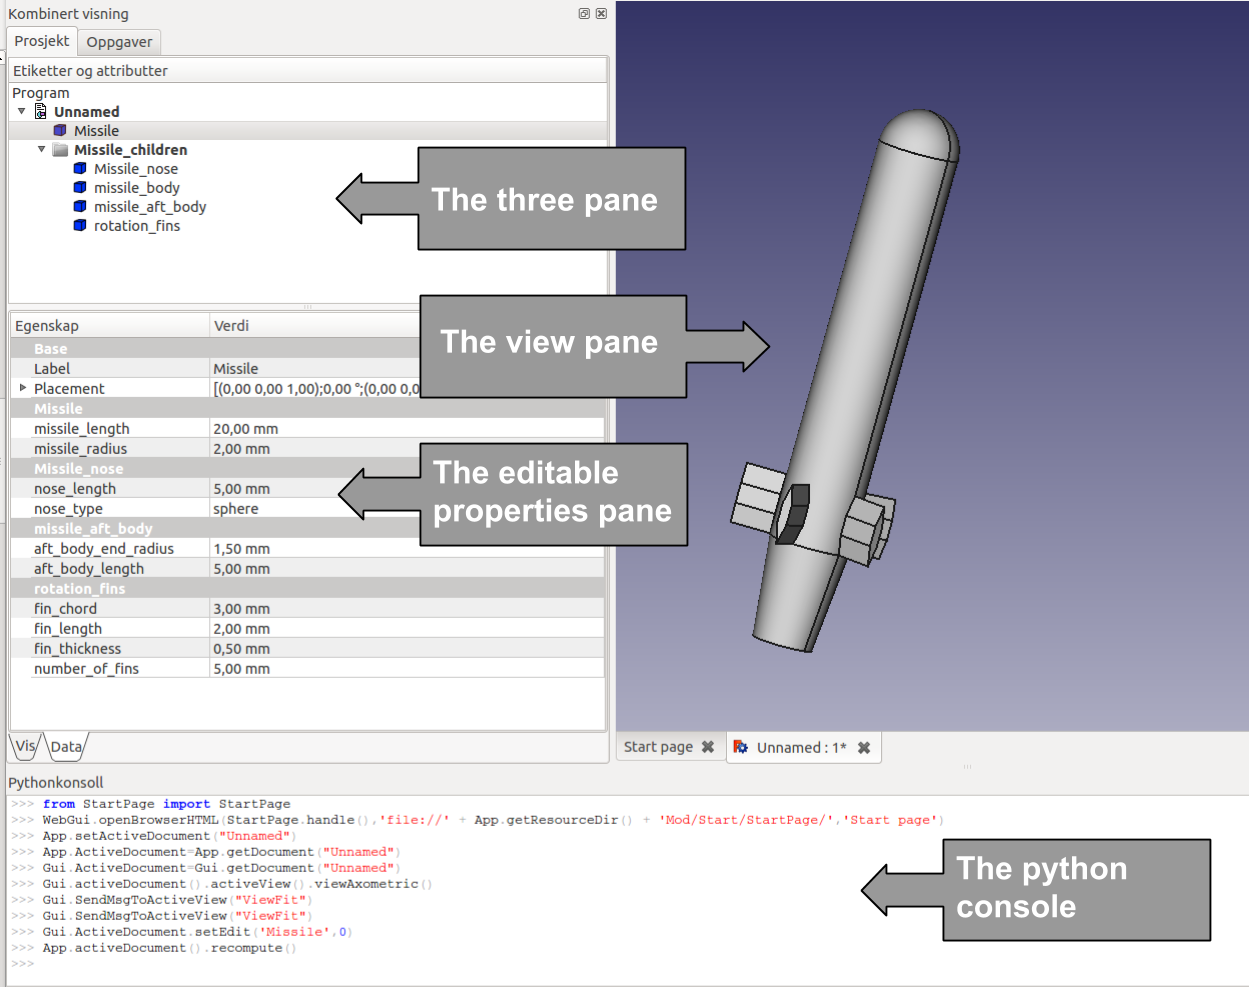
\includegraphics[width=120mm]{gfx/freecad_visulization.png}

\caption{The freeCAD graphical viewer visualizing the missile, with the three pane, editable properties pane, view-port pane and a Python console}
\label{fig:freecad}
\end{figure}
% subsubsection interfacing_with_aml_from_the_console (end)


\subsubsection{Testing support} % (fold)
\label{ssub:testing_support}
Testing is the practice of making objective judgments regarding the system's quality and correctness. It is a huge help for maintaining and developing a code base \citep{agile_samurai}. Testing big and complex structures, like KBE models, are not a easy task. Many problems tend to arise, because the different objects in the system have many complex dependencies between them \citep{aunit}. In the software industry this is solved with good testing frameworks and mocking. Mocking is done my creating mock objects, which are injected to isolate different objects from each other during testing. Mock objects are simulated objects that mimic the behavior of real objects in controlled ways. By using mock objects, we can assure that errors in one object does not affect the test results for another object. This makes locating errors and writing tests easier on complex systems, like KBE models.

Integrating a test framework in a KBE system, means that we have to isolate the models and their logic. In our case this implies we have to isolate the KbePart objects. They alone, hold all logic and rules governing the model and their geometry. With KbePart being a complete Python module, it is easy to integrate any test framework supported by the Python programming language.

Python have a large variety of test frameworks to choose from. Some varieties are unittest, pyUnit, py.test or doctest. They all have positive and negative qualities. We have chosen unittest, as this is the currently most used testing framework for Python.

Integrating the unittest framework was done in a normal manner. We imported the module and created a test case class.

\begin{python}[caption={Creating a TestCase},label={lst:test_case}]
  import unittest
  from mock import Mock

  class DescribeMissile(unittest.TestCase):

    def setUp(self):
        self.missile_doc = DocumentMock()
        self.missile = Missile(self.missile_doc)
        self.fp = FeaturePythonMock()
\end{python}

The \textit{setUp} function is called before each test is executed. We make the missile from independent from its dependencies, by creating two different mock objects, as we can see from the code snippet above and in Appendix~\ref{app:missile_spec.py}. The document mock simulates the freeCAD document where every model is added. The FeaturePythonMock is an object that represent all properties, so we can control them in the test situation. Every KbePart have control of its own objects, making it easy to abstract the parts currently being tested. Now we can start to make some tests. The first test, shown in Listing~\ref{lst:test_1}, is checking if the missile has four children.

\begin{python}[caption={Missile test 1},label={lst:test_1}]
   def test_missile_should_be_init_with_4_children(self):
        children_length = len(self.missile.children)
        self.assertEqual(children_length, 4)
 \end{python}

We are also able to mock out the objects/attributes/functions we want. Listing~\ref{lst:test_2} shows how we have mocked out the missile's execute function.

\begin{python}[caption={Missile test 2},label={lst:test_2}]
    def test_missile_should_update_when_a_value_is_changed(self):
        self.fp.missile_radius = 5
        self.missile.execute = Mock(return_value=True)
        self.missile.onChanged(self.fp, 'missile_radius')
        self.assertTrue(self.missile.execute.called)
\end{python}
% subsubsection testing_support (end)


\subsubsection{Debugging support} % (fold)
\label{ssub:debugging_support}
A lot of different debugging tools are available for the Python programming language. Some examples are WinPDB, PyDebug which are embedded in many Python IDEs. The most basic debugger is the Python debugger, which is available as a Python module called pdb. At the core this is a command line debugger, but there exists graphical interface that work with it. It also integrates with the Sublime Text 2 editor. It is integrated just by importing the pdb module. A breakpoint as created by inserting a \textit{pdb.set\_trace()}. When the code is executed, the developer is free to access all the debugger features through the command palette in Sublime, see Figure~\ref{fig:sublime_ide}.
% subsubsection debugging_support (end)

\subsubsection{IDE support} % (fold)
Many IDE options exist for Python. Some of the most acclaimed are PyCarm, Eclipse with PyDev, Wing and Sublime Text. We chose to integrate our it in sublime text, since it is our favorite editor, has a great variety of features and makes a nice comparison to our Sublime AML integration.

To better configure Sublime to Python editing, the anaconda \citep{anaconda} plug-in should be used. Anaconda adds a wide spectrum of facilities, like auto-complete, goto definition, goto documentation, refactoring, linting and much more. It also adds a lot of handful snippets.

To integrate Python debugger, the plug-in SublimeREPL was used. SublimeREPL is able to run a Python interpretor in a Sublime buffer. SublimeREPL has a command to run current file in pdb-mode, which is useful for debugging.

Sublime supports unit-testing out of the box. \textit{Ctrl+b}, compiles and runs the current test file. A little buffer at the bottom of the editor will pop up and display the test results, as shown in Figure~\ref{fig:sublime_ide}.

\begin{figure}[ht!]
\centering
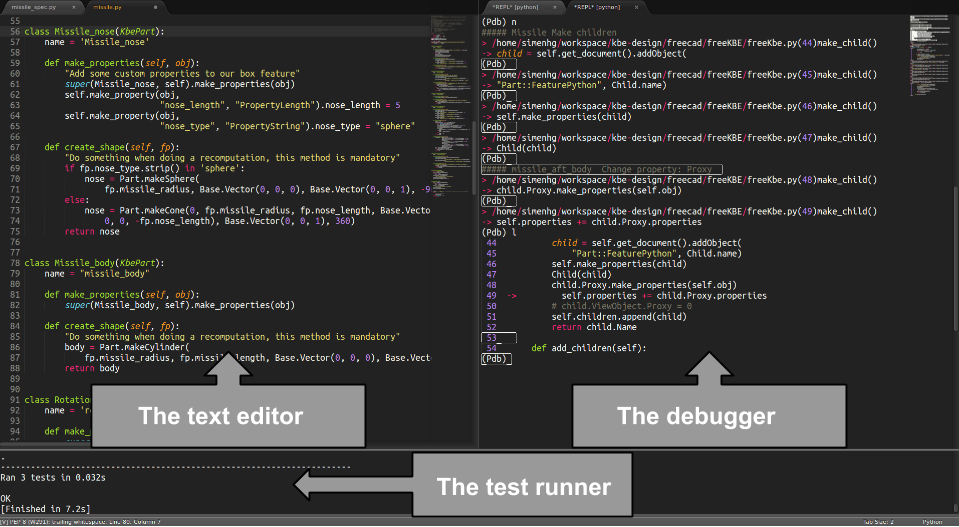
\includegraphics[width=120mm]{gfx/sublime_ide_arrows.png}

\caption{Sublime text integration, displaying the test runner, the debugger and the text editor.}
\label{fig:sublime_ide}
\end{figure}
% subsubsection ide_support (end)
% subsection integrating_general_software_tool (end)


\subsection{Problems with switching KBE-system} % (fold)
\label{sub:problems_with_switching_KBE_system}
In this chapter we have created a minimal KBE system and integrated a set of general software tools. In our tests, no major obstacles have been encountered. However, this is not conclusive evidence that creating a new KBE-system is an easy task.

Despite the fact that creating a new KBE System seems like a easy solution, some major problems has to be solved. One problems is continuation of knowledge. Today all knowledge and logic connected to a KBE model is interleaved in the KBE classes. This means that all knowledge is lost if one decide to switch KBE system. The knowledge can, however, be transferred to a new KBE system. It can for example be done by parsing the objects to the new system. It should be said that this is not an easy task and should be examined before attempting to create a new KBE system.

Time and quality is also factors we need to take into account. Although it is easy to integrate general software tools in a new KBE system, it may not be the best solution. The time it takes to create a good KBE system may exceed the time to integrate general software tool. The quality of a new system may also not be as good as a old and fully tested system.
% subsection problems_with_switching_KBE_system (end)
% section building_a_KBE_system (end)

%!TEX root = ../main.tex

\section{Results and discussion} % (fold)
\label{sec:discussion}

\subsection{Interfacing with AML, developing a new editor and exploring new learning possibilities} % (fold)
\label{sub:interfacing_with_aml_developing_a_new_editor_and_exploring_new_learning_possibilities}
Section 3.1, contained an exploration of the possibilities for interfacing with AML from the system console and from another programming language. The console interface of AML was initially hard to work with, compared to the general programming languages Python and Common Lisp. The reason was mostly because the lack of documentation and the slightly laborious setup needed to launch the AML process in the console. However, improving the documentation, could make the difference negligible.

Then the possibility of controlling AML from another programming language was addressed. Several attempts at making a prototype REPL for AML in Python was made, however only two of the attempts where successful. Reading and writing to the AML process in different threads and using a pseudo-TTY. This was doe to AML utilizing block-buffered IO when being piped to another process. An argument was made, that this behavior is caused by the way the C standard IO library behaves.

This behavior made interfacing with AML from other programming languages unnecessary hard, and it was reviled that other programming languages avoids the problem, by giving the user the option of forcing line-buffered or unbuffered IO. Making such options part of AML would be a valuable feature.

In section 3.2, the RQ~\ref{rq:structure_aml} was studied by making a prototype integration of AML into the Sublime Text 2 editor. Using the strategy of configuring the editors existing Common Lisp support to work with AML, and then integrating the AML console into the editor, gave a working prototype. This prototype was further enhanced by some general configuration of Sublime, in the end, managing to duplicate the most important features of the AML XEmacs integration.

The main drawback of the prototype AML integration, was the problems related to controlling the AML process from Python, as described in section 3.1. If AML had the option of line-buffered or unbuffered IO, the entire integration could have been made using configuration of existing features and plug-ins of Sublime.

Even with the problems related to integrating the AML console, development of the Sublime integration was fairly straight forward. With the prototype integration only a minimum development and maintenance is needed, although both the quality and maintainability of the console integration is diminished to some degree.

%TODO: ref to "an argument was made"....below
The next question, RQ~\ref{rq:another_editor}, was not covered in as great depth as the first one, mainly due to the difficulty of integrating the AML console. An argument was made for the value of choice between editors, something that in a sense can be understood as a feature not readily available in XEmacs. A brief overview of notable features in Sublime was supplied. Although some of these features can be duplicated in XEmacs, XEmacs being a highly configurable editor, the focus was to investigate the features readily available in the editor. With this premise one can argue that a Sublime AML integration offers other features than XEmacs.

In the section 3.3, the learning challenges of AML where addressed, and the learning material of AML was discussed. Some shortcomings of the current learning material for AML was addressed, and the option of using learning material designed for Common Lisp was explored with good results. Finally the benefits of having an active on-line community during the learning process was also discussed.

This section leads to the question if the syntax of AML should be made more closely like, or even compatible with, the syntax of ANSI compliant Common Lisp. This would give the developer even more options to use previously written general software tools together with AML. Our learning experience with AML indicated that even with the existing, non ANSI compliant syntax, AML training can be improved by using the learning material and community support for Common Lisp. By making the syntax ANSI compliant, further gains from this strategy is expected, and this could give the developer the option of using existing software libraries and tools written for Common Lisp.

The trade-of of altering the syntax in such a way, is compatibility with previous versions of AML, as well as the more substantial resources needed to modify the AML modeling system. These would be needed to be throughly investigated in a more if such an undertaking was to be considered, but the possible gains of making this change makes us recommend that this should be studied in further work.
% subsection interfacing_with_aml_developing_a_new_editor_and_exploring_new_learning_possibilities (end)

\subsection{Building KBE models with Python and Open CASCADE} % (fold)
\label{sub:building_kbe_models_with_python_and_open_cascade}
In the introduction, another way of integrating GSD tools was introduced and the RQ~\ref{rq:intgenssofttools} was submitted.

The anatomy of a KBE system and different options for replacing the individual components was discussed, before settling with Python as the programming language, and Open CASCADE and FreeCAD for the geometric kernel and graphical viewer.

A test model of the missile system, described in the AML basic training manual, was developed. To aid with developing the model, ready made solutions for IDE, testing and debugging support was utilized. Compared to the troubles faced when developing the Sublime AML integration, this indicates that integrating general software tools is easier when the KBE-system is based on a widely used programming language.

More surprisingly, using this system to develop KBE models, was not as complicated as initially estimated, much due to the large amount of available open source tools and libraries. Notable drawbacks of using such a system was also identified in Section~\ref{sub:problems_with_switching_KBE_system}.
% subsection building_kbe_models_with_python_and_open_cascade (end)
% section discussion (end)


\section{Conclusion} % (fold)
\label{sec:conclusion}
The success of extending AML with parts from general software tools was in our cases largely dependent on the interfacing options to access AML from other programming languages. Documenting the console interface and allowing to force unbuffered or line buffered IO would have made the task of integrating AML into Sublime a trivial task, well within the grasp of a beginning KBE developer with some programming experience. It is our belief that this will enable developers to integrate AML into their favorite development tools, diversifying and expanding the AML system.

Documenting the console interface and allowing to force unbuffered or line buffered IO, seems to be possible to implement in AML without huge alterations to the existing framework.

Further modifications could be made to give AML a ANSI compatible syntax, giving AML developers even greater gain from using Common Lisp learning material as well as access to previously written libraries and tools for the more widely used Common Lisp language. If this where to be considered as an option, further investigation should be preformed, due to the possible complexities related to such modifications. Either way, resources used by Thecnosoft on developing learning material, might be better used on expanding the material covering KBE-specific parts of AML, and use learning material for Common Lisp to teach the basics of Lisp languages.

By experimenting with building KBE models with a widely used programming language, we instantly got access to testing, debugging and IDE/editor support. This we feel, demonstrates the advantages of having a KBE system that is compatible with general software tools. The obstacles of using such an approach is also apparent. Development time, quality, knowledge transfer from old systems, all makes this a more substantial undertaking than one might believe at first glance.

The ease of building KBE models with existing general software tools, should be seen as an incentive for Technosoft to push for better access to AML from other programming languages. Using a widely used general programming language at the core of a KBE model, instantly gives the developer access to a large amount of existing development tools, libraries and training material. Although development of KBE models with existing general software tools is not an viable alternative to AML today, this might change in the future. In such a scenario, changes would be needed to make AML an competitive option for the KBE developer.

To conclude this report, the authors would like to inform the reader that all code written as part of this project is freely available for use, re-use and sharing at \url{https://github.com/teodoran/TDT-4560}. An video-tutorial AMLRepl is available at \url{https://www.dropbox.com/s/5n2ksllro5kj72o/aml-repl-tutorial.mpg}.
% section conclusion (end)
% include content
%\include{./tex/test}

% References
% Add a ''References`` entry in TOC
\addcontentsline{toc}{section}{References}
\bibliographystyle{plain}
\bibliography{./bib/refbib}

% Appendix, starts on an odd-numbered page
\cleardoublepage
% Appendix uses plain style (only page numbers)
\pagestyle{plain}
% start appendix
\begin{appendices}
\appendix
%!TEX root = ./main.tex
\section*{\begin{center}{\Huge Appendix}\end{center}}
\addcontentsline{toc}{chapter}{Appendix}
\vspace{1 cm}

\noindent Write your appendix here\dots


\section{Brute Force - Garcia} % (fold)
\label{sec:brute_force_garcia}

% section brute_force_garcia (end)

\section{Radix select} % (fold)
\label{sec:radix_select}

% section radix_select (end)
 \section{Parallel quick select} % (fold)
 \label{sec:parallel_quick_select}

 % section parallel_quick_select (end)

\section{Paralell k-d tree build} % (fold)
\label{sec:paralell_k_d_tree_build}

% section paralell_k_d_tree_build (end)


\section{Multiple radix select} % (fold)
\label{sec:multiple_radix_select}

% section multiple_radix_select (end)

\section{CUDA-K-d tree search} % (fold)
\label{sec:cuda_k_d_tree_search}

% section cuda_k_d_tree_search (end)

\section{OpenMP - K-d tree search} % (fold)
\label{sec:open_mp_k_d_tree_search}

% section k_d_tree_search_das_openmp (end)

\end{appendices}

\end{document}
